\documentclass[10pt]{beamer}
\usepackage{physics}
\usepackage{amsfonts}
\usepackage{amsmath}
\usepackage{graphicx}
\graphicspath{{../images/}}
\usepackage[utf8]{inputenc}
\usetheme{Warsaw}
\usepackage[style=verbose]{biblatex}
\addbibresource{../References.bib}
\usepackage[justification=centering]{caption}
\captionsetup[figure]{labelformat=empty}
\useoutertheme{infolines}
\setbeamertemplate{navigation symbols}{}
%\setbeamertemplate{headline}{}
\usecolortheme{default}
\setbeamerfont{subsection in toc}{size=\small}
\setbeamerfont{footnote}{size=\tiny}
\expandafter\def\expandafter\insertshorttitle\expandafter{%
  \insertshorttitle\hfill%
  \insertframenumber\,/\,\inserttotalframenumber}
\title[E213 : Analysis of Decays of heavy vector boson $\rm Z^{0}$] %optional
{E213 : Analysis of Decays of heavy vector boson $\rm Z^{0}$}
\author[Sakthivasan, Jena] % (optional)
{Group P20: Ajay Shanmuga Sakthivasan \& Mrunmoy Jena\\
Supervisor: Martin Angelsmark}


\date{\today}

\begin{document}
\begin{frame}
    \titlepage 
\end{frame}

\begin{frame}
    \frametitle{Outline}
    \tableofcontents
\end{frame}

\section{Introduction}
\begin{frame}
\frametitle{Introduction}
\begin{itemize}
\item Goal: to understand how data from a particle accelerator is analysed and to deduce different properties of the $Z^0$ boson
\item Important physical quantities: $Z^0$ mass and decay width 
\item Data collected from the OPAL (Omni-Purpose Apparatus at LEP) detector
\item Part I: Carried out event display analysis on smaller datasets to understand how to separate out different $Z^0$ decay channels
\item Part II: Cuts (constraints) imposed on the data are refined and statistical analysis done on larger real world data $\rightarrow$ deduce physical quantities
\end{itemize}
\end{frame}
\section{Prerequisite Knowledge}
\subsection{Standard Model}
\begin{frame}
\frametitle{Standard Model}
\begin{minipage}{0.5\textwidth}
\begin{itemize}
\item Standard Model: provides the most fundamental description of nature by incorporating the elementary particles and their interactions
\item Two families: fermions (half integer spins), and bosons (integer spins)
\begin{itemize}
\item EM interactions $\rightarrow$ photon ($\gamma$)
\item Strong force $\rightarrow$ gluons (g) 
\item Weak force $\rightarrow$ $W^{\pm}, Z^{0}$ 
\item Gravity $\rightarrow$ graviton (hypothesized; not included in SM)
\end{itemize}
\end{itemize}
\end{minipage}\hspace{2em}
\begin{minipage}{0.35\textwidth}
      \begin{figure}
      \centering
        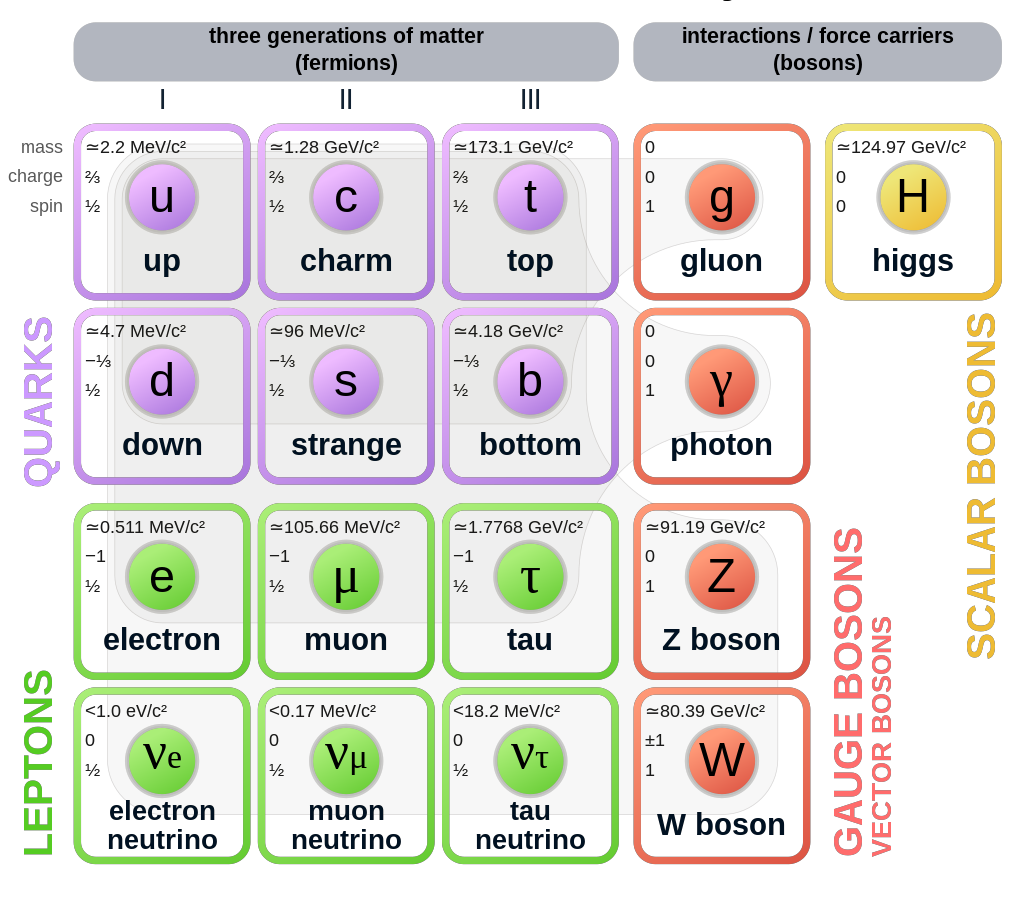
\includegraphics[height=\textwidth]{Standard_Model_of_Elementary_Particles}
        \caption{Standard Model \footnotemark{}}
      \end{figure}
  \end{minipage}\hfill
  \footcitetext{stdmodel}
\end{frame}
\begin{frame}
\frametitle{Standard Model}
\begin{itemize}
\item Fermions: three generations of quarks and leptons
\begin{itemize}
\item Six flavours of quarks: up (u), down (d), charm (c), strange (s), top (t) and bottom (b)
\item Six flavours of leptons: electron ($e$), muon ($\mu$) and tau ($\tau$), and associated neutrinos ($\nu_{e}$, $\nu_{\mu}$ and $\nu_{\tau}$)
\end{itemize}
\item Composite particles: three quark combinations, called baryons ($qqq$/$\bar{q}\bar{q}\bar{q}$) or quark-antiquark pairs, called  mesons ($q\bar{q}$)
\item Mathematically, elementary particles $\rightarrow$ elements of representations of certain symmetry groups
\item Gauge fields coupling to these particles $\rightarrow$ consequence of invariance of corresponding Lagrangian under local phase transformations \footnotemark{}
\item Gauge symmetry that governs the Standard Model is given by: $$SU(3)_{\mathrm{Colour}}\times SU(2)_{\mathrm{Left\ chiral}}\times U(1)_{\mathrm{Y}(\mathrm{Weak \ hypercharge})}$$
\end{itemize}
\footcitetext{thomson_2013}
\end{frame}
\subsection{Electroweak Theory}
\begin{frame}
\frametitle{Electroweak Theory}
\begin{itemize}
\item Initially, EM and the theory of weak interactions formulated separately
\item At higher energies ($\sim$ 246 GeV \footnotemark{}), unified into single force $\rightarrow$ GSW electroweak model - 1960s
\item Impose local gauge invariance on $SU(2)_{L}$ symmetry group $\rightarrow$ three gauge fields: $W^{(1)},\ W^{(2)}$ and $W^{(3)}$
\item Physical $W^{+}$ and $W^{-}$ bosons found to be linear combinations: 
\begin{equation}
W^{\pm}_{\mu}=\dfrac{1}{\sqrt{2}}\left(W^{(1)}_{\mu}\mp \rm{i}W^{(2)}_{\mu}\right)
\end{equation}
\end{itemize}
\footcitetext{pdg-ew}
\end{frame}

\begin{frame}
\frametitle{Electroweak Theory}
\begin{itemize}
\item $W^{(3)}_{\mu}$ field (no physical interpretation ?)
\item Additional symmetry, the $U(1)_{Y}$ group is introduced
\item $B_{\mu}$ field arising from $U(1)_{Y}$ symmetry (no physical meaning ?)
\item Linear combinations of $W^{(3)}_{\mu}$ and $B_{\mu}$ fields $\rightarrow$ photon and the $Z^{0}$ boson:

\begin{equation}
\begin{pmatrix} 
A_{\mu} \\ 
Z_{\mu} 
\end{pmatrix}
= 
\begin{pmatrix}
\cos \theta_{W} & \sin \theta_{W} \\
-\sin \theta_{W} & \cos \theta_{W} 
\end{pmatrix}
\begin{pmatrix}
B_{\mu} \\
W^{(3)}_{\mu}
\end{pmatrix}
\end{equation}
$\theta_{W}$ : weak mixing/Weinberg angle
\end{itemize}
\end{frame}
\subsection{Physics Related to the $Z^{0}$ Resonance}
\subsubsection{$e^{+}e^{-}$ Interactions}
\begin{frame}
\frametitle{$e^{+}e^{-}$ Interactions}
\end{frame}
\subsubsection{Forward-Backward Asymmetry}
\begin{frame}
\frametitle{Forward-Backward Asymmetry}
\end{frame}
\subsubsection{Background Processes: Radiative Corrections}
\begin{frame}
\frametitle{Background Processes: Radiative Corrections}
\end{frame}
\subsubsection{Breit Wigner Distribution}
\begin{frame}
\frametitle{Breit Wigner Distribution}
\end{frame}
\subsubsection{LEP Experiment and OPAL Detector}
\begin{frame}
\frametitle{The LEP Experiment}
\end{frame}
\begin{frame}
\frametitle{OPAL Detector and its Components}
\end{frame}
\section*{References}
\begin{frame}
\frametitle{References}
\printbibliography
\end{frame}
\end{document}